% !TEX root = ../master/master.tex

%% Dexter Barrows, 2016
%% dbarrows.github.io

\section{Fitting Setup}

	Now that we have established which methods we wish to evaluate the efficacy of for epidemic forecasting, it is prudent to see how they perform when fitting parameters for a known epidemic model. We have already seen how they perform when fitting parameters for a model with a deterministic evolution process and observation noise, but a more realistic model will have both process and observation noise.

	To form such a model, we will take a deterministic SIR ODE model specified in Equation [\ref{sirode}] and add process noise by allowing $\beta$ to follow a geometric random walk given by

	\begin{equation}\label{betaautoreg}
		\beta_{t+1} = \exp \left( \log(\beta_{t}) + \eta (\log(\bar{\beta}) - \log(\beta_{t})) + \epsilon_{t} \right).
	\end{equation}

	We will take $\epsilon_{t}$ to be normally distributed with standard deviation $\rho^2$ such that $\epsilon_{t} \sim \mathcal{N}(0,\rho^2)$. The geometric attraction term constrains the random walk, the force of which is $\eta \in [0,1]$. If we take $\eta = 0$ then the walk will be unconstrained; if we let $\eta = 1$ then all values of $\beta_t$ will be independent from the previous value (and consequently all other values in the sequence).

	When $\eta \in (0,1)$, we have an autoregressive process of order 1 on the logarithmic scale of the form

	\begin{equation}
		X_{t+1} = c + \rho X_t + \epsilon_t ,
	\end{equation}

	where $\epsilon_t$ is normally distributed noise with mean 0 and standard deviation $\sigma_E$. This process has a theoretical expected mean of $\mu = c / (1 - \rho)$ and variance $\sigma = \sigma_E^2 / (1 - \rho^2)$. If we choose $\eta = 0.5$, the resulting log-normal distribution has a mean of $6.80 \times 10^{-4}$ and standard deviation of $4.46 \times 10^{-4}$.

	Figure [\ref{betaplot}] shows the result of simulating the process in Equation [\ref{betaautoreg}] with $\eta = 0.5$.

	\begin{figure}
        \centering
        \captionsetup{width=.8\linewidth}
        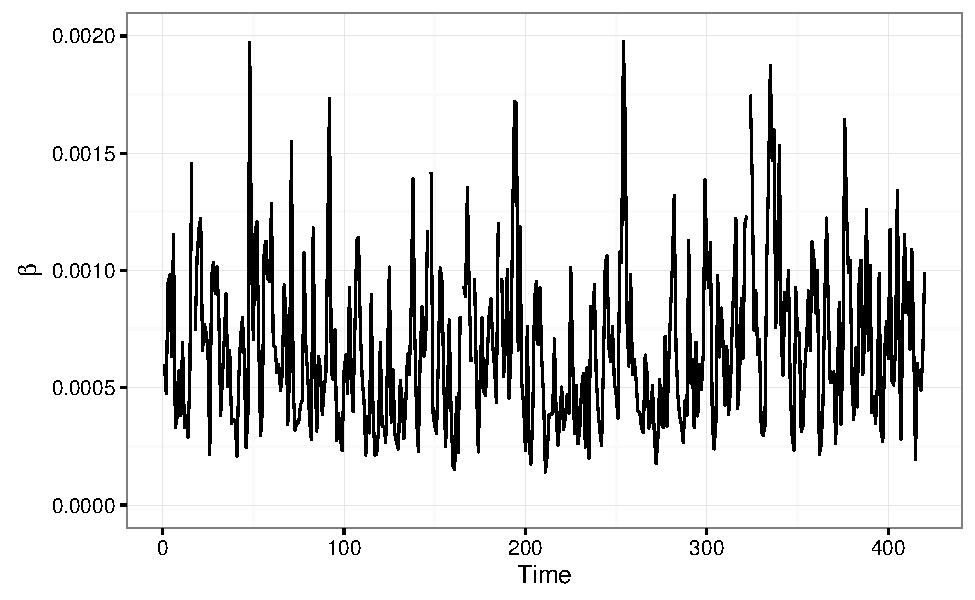
\includegraphics[width=0.8\textwidth]{./images/betaplot.pdf}
        \caption{Simulated geometric autoregressive process shown in Equation [\ref{betaautoreg}]. \label{betaplot}}
    \end{figure}

    Figure [\ref{betadensity}] shows the density plot corresponding to the values in Figure [\ref{betaplot}].

    \begin{figure}
        \centering
        \captionsetup{width=.8\linewidth}
        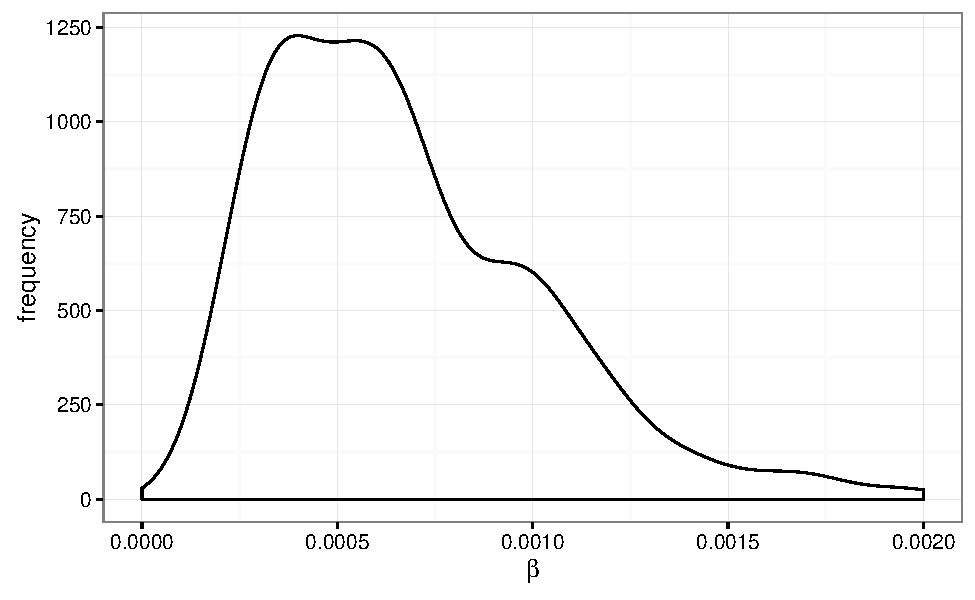
\includegraphics[width=0.8\textwidth]{./images/betadensity.pdf}
        \caption{Density plot of values shown if Figure[\ref{betaplot}]. \label{betadensity}}
    \end{figure}

    We see a density plot similar in shape to the desired density, and the geometric random walk displays dependence on previous values. Further the mean of this distribution was calculated to be $6.92 \times 10^{-4}$ and standard the deviation to be $3.99 \times 10^{-4}$, which are very close to the theoretical values.

    If we take the full stochastic SIR system and evolve it using an Euler stepping scheme with a step size of $h = 1/7$, for 1 step per day, we obtain the plot in Figure [\ref{sirmean}].

    \begin{figure}
        \centering
        \captionsetup{width=.8\linewidth}
        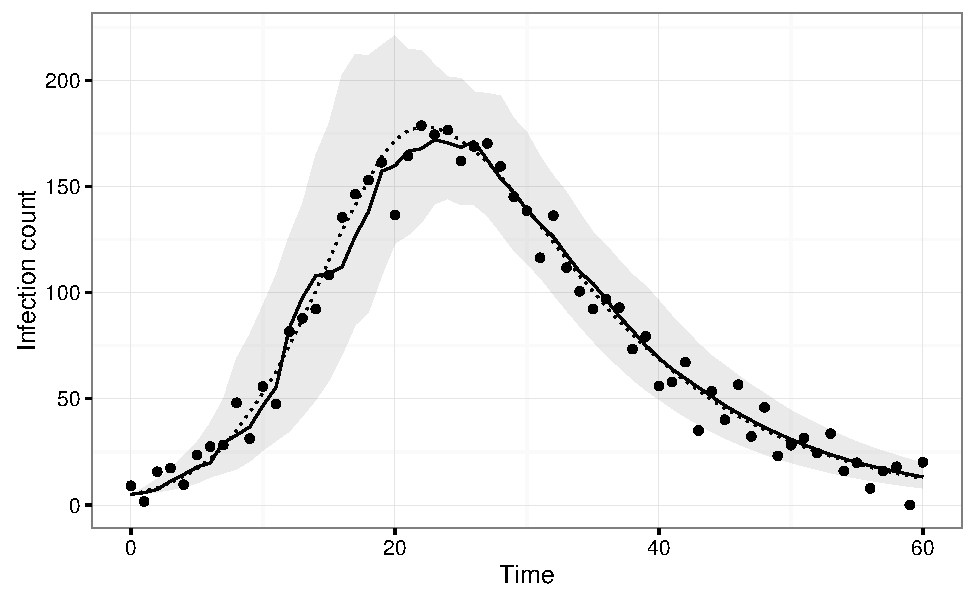
\includegraphics[width=0.8\textwidth]{./images/sirmean.pdf}
        \caption{Stochastic SIR model simulated using an explicit Euler stepping scheme. The solid line is a single random trajectory, the dots show the data points obtained by adding in observation error defined as $\epsilon_{\small\text{obvs}} = \mathcal{N}(0,10)$, and the grey ribbon is centre 95th quantile from 100 random trajectories. \label{sirmean}}
    \end{figure}


\section{Calibrating Samples}

	In order to compare HMC and IF2 we need to set up a fair and theoretically justified way to select the number of samples to draw for the HMC iterations and the number of particles to use for IF2. As we wish to compare, among other things, approximate computational cost using runtimes, we need to determine how many sample draws for each method are required to obtain a certain accuracy. Sample draws are typically not comparable in terms of quality when considering multiple methods. For example, vanilla MCMC draws are computationally cheap compared to those from HMC, but HMC produces draws that more efficiently cover the sampling space. Thus we cannot just set the number of HMC draws equal to the number of particles used in IF2 -- we must calibrate both quantities based on a desired target error. We assume that we are working with a problem that has an unknown real solution, so we use the Monte Carlo Standard Error (MCSE) \cite{Harding2014}.

	Suppose we are using a Monte-Carlo based method to obtain a mean estimate $\hat{\mu}_{n}$ for a quantity $\mu$, where $n$ is the number of samples. Then the Law of Large Numbers says that $\hat{\mu}_{n} \rightarrow \mu$ as $n \rightarrow \infty$. Further, the Central Limit Theorem says that the error $\hat{\mu}_{n} - \mu$ should shrink with number of samples such that $\sqrt{n} (\hat{\mu}_{n} - \mu) \rightarrow \mathcal{N}(0,\sigma^2)$ as $n \rightarrow \infty$, where $\sigma^2$ is the variance of the samples drawn.

	We of course do not know $\mu$, but the above allows us to obtain an estimate $\hat{\sigma}_n$ for $\sigma$ given a number of samples $n$ as

	\begin{equation}
		\hat{\sigma}_n = \sqrt{\frac{1}{n} \sum_{i=1}^{n} (X_i - \hat{\mu}) },
	\end{equation}

	which is known as the Monte Carlo Standard Error.

	We can modify this formula to account for multiple, potentially correlated, variables by replacing the single variance measure sum by

	\begin{equation}
		\Theta^* V (\Theta^*)^T
	\end{equation}

	where $\Theta^*$ is a row vector containing the reciprocals of the means of the parameters of interest, and $V$ is the variance-covariance matrix with respect to the same parameters. This in effect scales the variances with respect to their magnitudes and accounts for covariation between parameters in one fell swoop. We also divide by the number of parameters, yielding

	\begin{equation}
		\hat{\sigma}_n = \sqrt{\frac{1}{n} \frac{1}{P} \Theta^* V (\Theta^*)^T }
	\end{equation}

	where $P$ is the number of particles.

	The goal here is to then pick the number of HMC samples and IF2 particles to yield similar MCSE values. To do this we picked a combination of parameters for RStan that yielded decent results when applied to the stochastic SIR model specified above, calculated the resulting mean MCSE across several model fits, and isolated the expected number of IF2 particles needed to obtain the same value. This was used as a starting value to ``titrate'' the IF2 iterations to the same point.

	The resulting values were 1000 HMC warm-up iterations with 1000 samples drawn post-warm-up, and 2500 IF2 particles sent through 50 passes, each method giving an approximate MCSE of 0.0065.


\section{IF2 Fitting}

	Now we will use an implementation of the IF2 algorithm to attempt to fit the stochastic SIR model to the previous data. The goal here is just parameter inference, but since IF2 works by applying a series of particle filters we essentially get the average system state estimates for a very small additional computational cost. Hence, we will will also look at that estimated behaviour in addition the parameter estimates.

	The code used here is a mix of R and C++ implemented using Rcpp. The fitting was undertaken using $2500$ particles with 50 IF2 passes and a cooling schedule given by a reduction in particle spread determined by $0.975^{p}$, where p is the pass number starting with 0. This geometric cooling scheme is standard for use with IF2 \cite{King2015a}\cite{King2016}, with the cooling rate chosen to neatly scale the perturbation factor from 1 to 0.02 (almost 0) over 50 passes.

	The MLE parameter estimates, taken to be the mean of the particle swarm values after the final pass, are shown in the table in Figure [\ref{fiterror}], along with the true values and the relative error.

	\begin{figure}
		\centering
		{\small
		\begin{tabular}{cccccc}
			& & \multicolumn{2}{c}{IF2} & \multicolumn{2}{c}{HMC} \\
			\cmidrule[1.0pt](r){3-4} \cmidrule[1.0pt](r){5-6}
			Name & True	& Fit & Error & Fit & Error \\
			\cmidrule[1.0pt](r){1-1} \cmidrule[1.0pt](r){2-2} \cmidrule[1.0pt](r){3-3} \cmidrule[1.0pt](r){4-4} \cmidrule[1.0pt](r){5-5} \cmidrule[1.0pt](r){6-6}
			$\mathcal{R}_0$ 		& 3.0 				 & 3.27 					& $9.08 \times 10^{-2}$ 	& $3.12$ 				& $1.05 \times 10^{-1}$		\\
			$\gamma$ 				& $10^{-1}$  		 & $1.04 \times 10^{-1}$ 	& $3.61 \times 10^{-2}$ 	& $9.99 \times 10^{-2}$ & $-7.56 \times 10^{-4}$	\\
			Initial Infected 	& 5  				 & 7.90 					& $5.80 \times 10^{-1}$ 	& $6.64$ 				& $3.28 \times 10^{-1}$ 	\\
			$\sigma$ 			& 10   				 & 8.84 					& $-1.15 \times 10^{-1}$ 	& $8.5$ 				& $-1.50 \times 10^{-1}$	\\
			$\eta$ 				& $5 \times 10^{-1}$ & $5.87 \times 10^{-1}$ 	& $1.73 \times 10^{-1}$ 	& $4.57 \times 10^{-1}$ & $-8.27 \times 10^{-2}$ 	\\
			$\varepsilon_{err}$ & $5 \times 10^{-1}$ & $1.63 \times 10^{-1}$ 	& $-6.73 \times 10^{-1}$ 	& $1.60 \times10^{-1}$  & $-6.80 \times 10^{-1}$
		\end{tabular}}
	    \caption{Fitting errors. \label{fiterror}}
    \end{figure}


	From last IF2 particle filtering iteration, the mean state values from the particle swarm at each time step are shown with the true underlying state and data in the plot in Figure [\ref{if2state}].

	\begin{figure}
        \centering
        \captionsetup{width=.8\linewidth}
        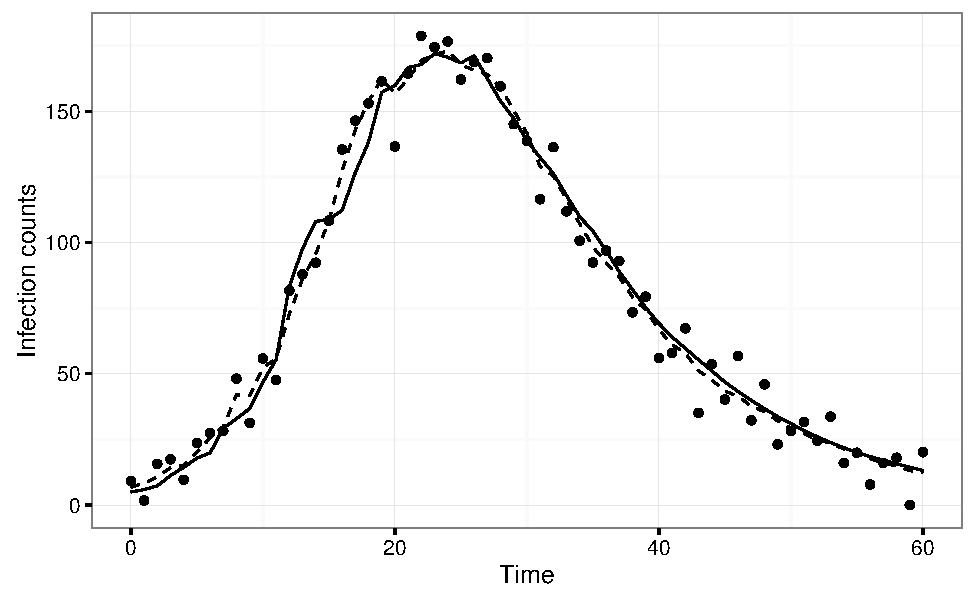
\includegraphics[width=0.8\textwidth]{./images/if2state.pdf}
        \caption{True system trajectory (solid line), observed data (dots), and IF2 estimated real state (dashed line). \label{if2state}}
    \end{figure}


\section{IF2 Convergence}

	Since IF2 is an iterative algorithm where each pass through he data is expected to push the parameter estimates towards the MLE, we can see the evolution of these estimates as a function of the pass number. We expect near-convergence in the parameter estimates as IF2 nears the maximum number of passes specified. Unconvincing convergence plots may signal suboptimal algorithm parameters. If sensible algorithm parameters have been chosen, we should see the convergence plots display ``flattening'' over time.

	Figure [\ref{if2convergence}] shows evolution of the mean estimates for the six most critical parameters.

	\begin{figure}
        \centering
        \captionsetup{width=.8\linewidth}
        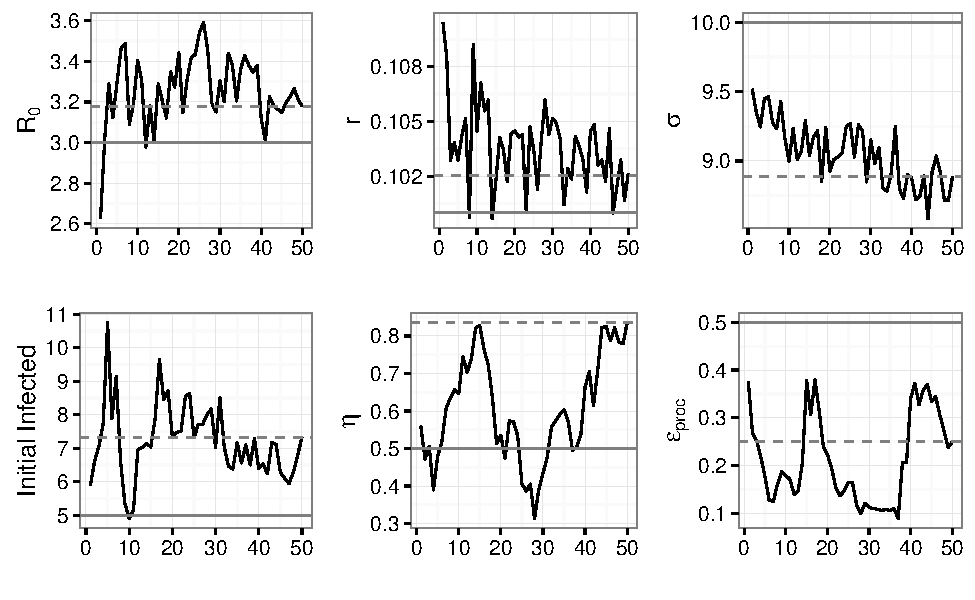
\includegraphics[width=0.8\textwidth]{./images/if2convergence.pdf}
        \caption{The horizontal axis shows the IF2 pass number. The solid black lines show the evolution of the ML estimates, the solid grey lines show the true value, and the dashed grey lines show the mean parameter estimates from the particle swarm after the final pass. \label{if2convergence}}
    \end{figure}

    Figure [\ref{if2sdconvergence}] shows the evolution of the standard deviations of the parameter estimates from the particle swarm as a function of the pass number. We should expect to see asymptotic convergence to zero if the filter is converging.

    \begin{figure}
        \centering
        \captionsetup{width=.8\linewidth}
        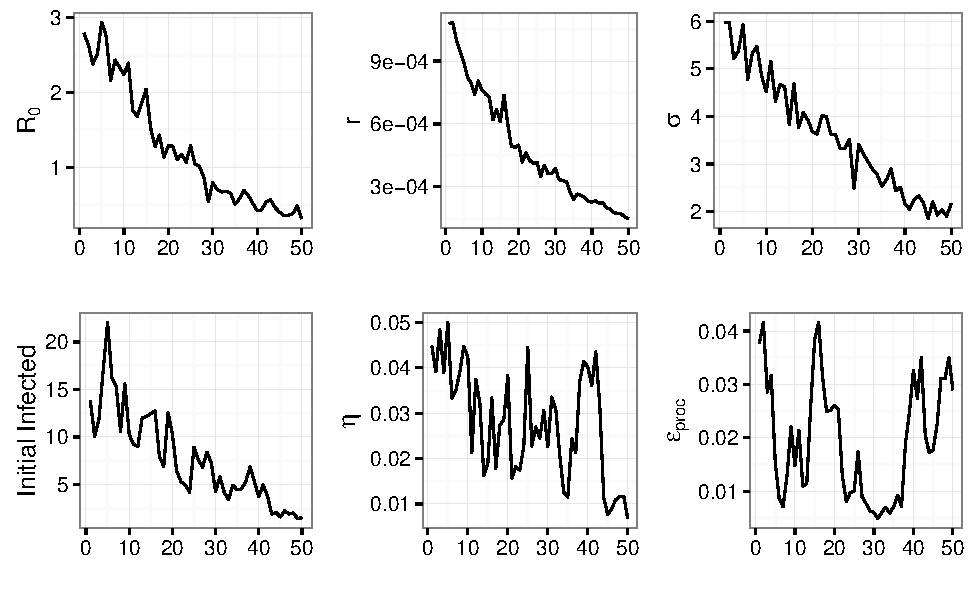
\includegraphics[width=0.8\textwidth]{./images/if2sdconvergence.pdf}
        \caption{The horizontal axis shows the IF2 pass number and the solid black lines show the evolution of the standard deviations of the particle swarm values. \label{if2sdconvergence}}
    \end{figure}


\section{IF2 Densities}

	Of diagnostic importance are the densities of the parameter estimates given by the final parameter swarm. If the swarm has collapsed, these densities will be extremely narrow, almost resembling a vertical line. A ``healthy'' swarm should display relatively smooth kernels of reasonable breadth.

	Figure [\ref{sc1if2kernels}] shows the parameter sample distributions from the final parameter swarm.

	\begin{figure}
        \centering
        \captionsetup{width=.8\linewidth}
        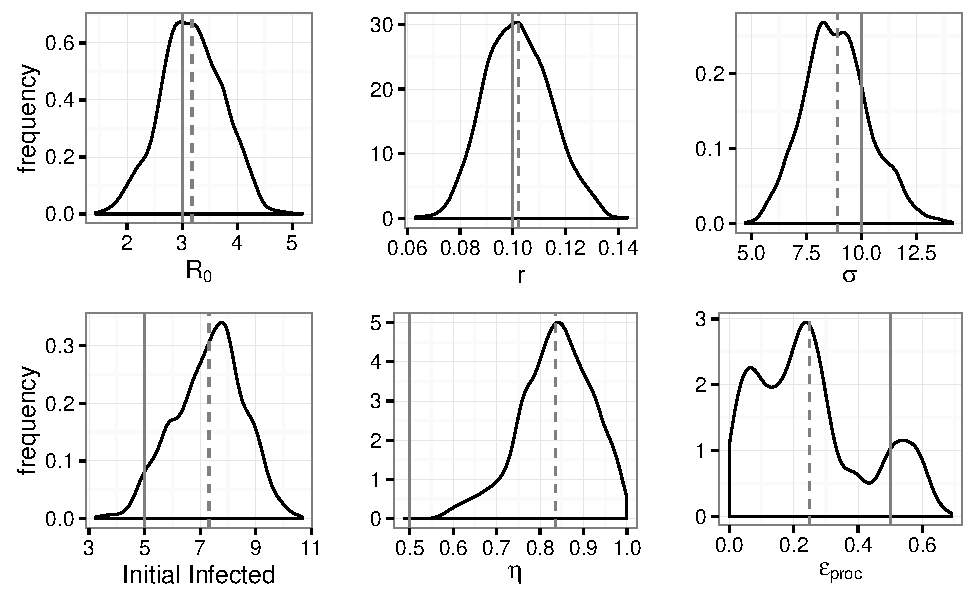
\includegraphics[width=0.8\textwidth]{./images/if2kernels.pdf}
        \caption{The solid grey lines show the true parameter values and the dashed grey lines show the density medians. \label{sc1if2kernels}}
    \end{figure}

    The IF2 parameters chosen were in part chosen so as to not artificially narrow these densities; a more aggressive cooling schedule and/or an increased number of passes would have resulted in much narrower densities, and indeed have the potential to collapse them to point estimates. This is undesirable as it may indicate instability -- the particles may have become ``trapped'' in a region of the sampling space.


\section{HMC Fitting}

	We can use the Hamiltonian Monte Carlo algorithm implemented in the RStan package to fit the stochastic SIR model as above. This was done with a single HMC chain of 2000 iterations with 1000 of those being warm-up iterations.

	The MLE parameter estimates, taken to be the means of the samples in the chain, were shown in the table in Figure [\ref{fiterror}] along with the true values and relative error.


\section{HMC Densities}

	Figure [\ref{sc1hmckernels}] shows the parameter estimation densities from the Stan HMC fitting.

	\begin{figure}
        \centering
        \captionsetup{width=.8\linewidth}
        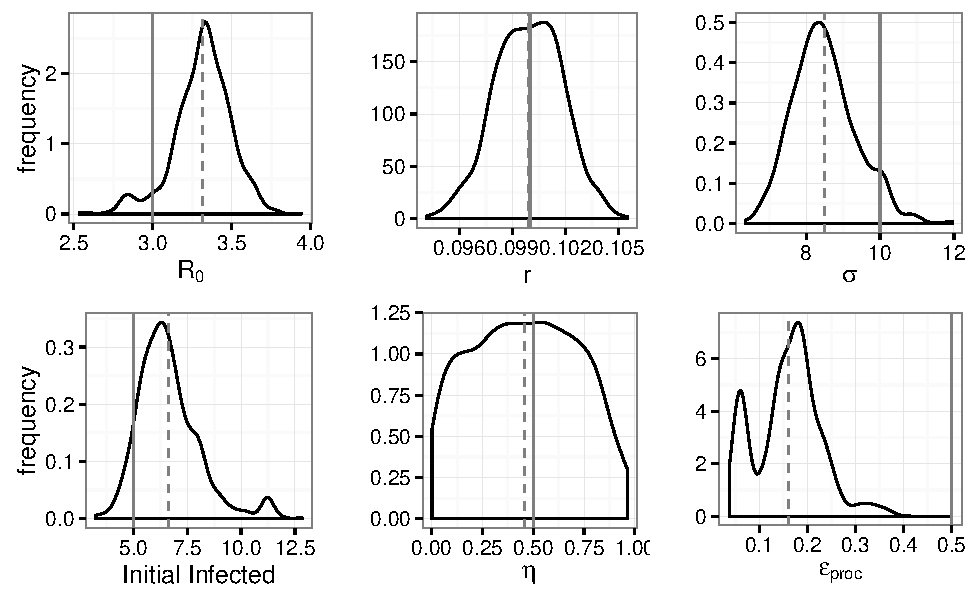
\includegraphics[width=0.8\textwidth]{./images/hmckernels.pdf}
        \caption{As before, the solid grey lines show the true parameter values and the dashed grey lines show the density medians. \label{sc1hmckernels}}
    \end{figure}

    The densities shown here represent a ``true'' MLE density estimate in that they represent HMC's attempt to directly sample from the parameter space according to the likelihood surface, unlike IF2 which is in theory only trying to get a ML point estimate. Hence, these densities are potentially more robust than those produced by the IF2 implementation.


\section{HMC and Bootstrapping}

	Unlike in some models, our RStan epidemic model does not keep track of state estimates directly, but does keep track of the autoregressive process latent variable draws, which allow us to reconstruct states. This was done to ease implementation as RStan places some restrictions on how interactions between parameters and states can be specified.

	Figure [\ref{hmcboot}] shows the results of 100 bootstrap trajectories generated from the RStan HMC samples.

	\begin{figure}
        \centering
        \captionsetup{width=.8\linewidth}
        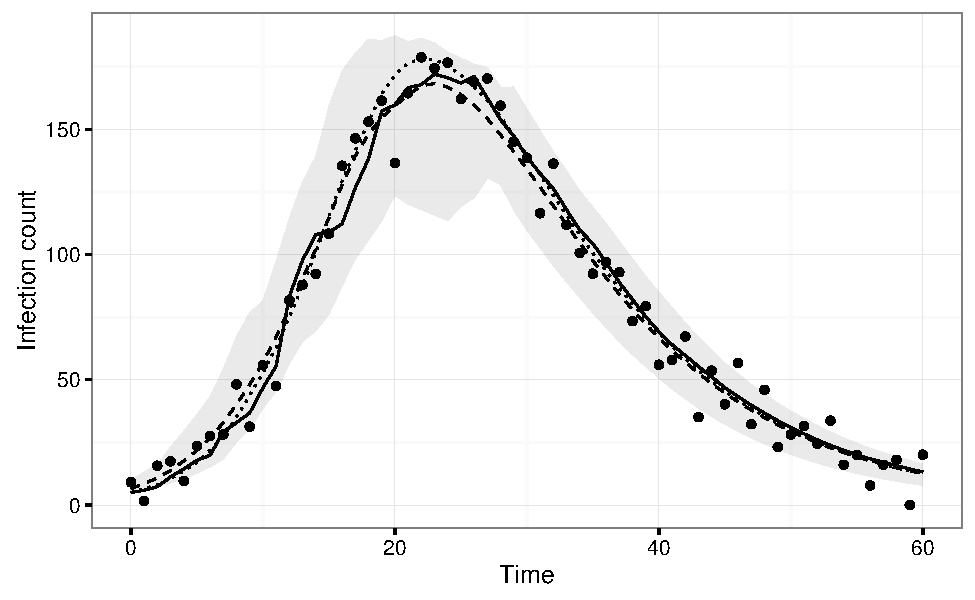
\includegraphics[width=0.8\textwidth]{./images/hmcboot.pdf}
        \caption{Result from 100 HMC bootstrap trajectories. The solid line shows the true states, the dots show the data, the dotted line shows the average system behaviour, the dashed line shows the bootstrap mean, and the grey ribbon shows the centre 95th quantile of the bootstrap trajectories. \label{hmcboot}}
    \end{figure}


\section{Multi-trajectory Parameter Estimation}

	Here we fit the stochastic SIR model to 200 random independent trajectories using each method and examine the density of the point estimates produced.

	Figure [\ref{combinedmulti}] shows the results of the mean parameter fits from IF2 and HMC for 200 independent data sets generates using the previously described model.

    \begin{figure}
        \centering
        \captionsetup{width=.8\linewidth}
        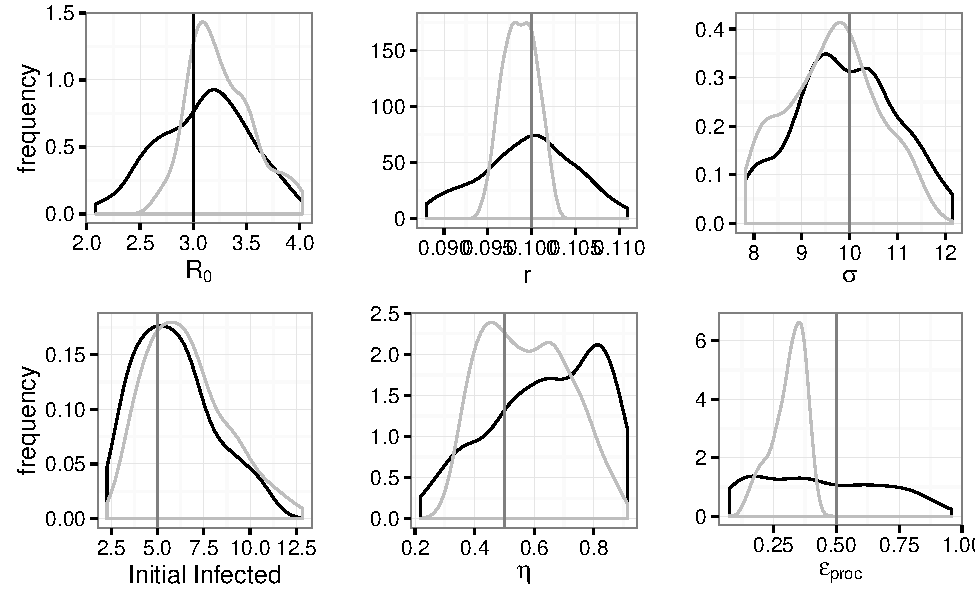
\includegraphics[width=0.8\textwidth]{./images/combined-multi.pdf}
        \caption{IF2 point estimate densities are shown in black and HMC point estimate densities are shown in grey. The vertical lines show the true parameter values. \label{combinedmulti}}
    \end{figure}

    The densities by and large display similar coverage, with the IF2 densities for $r$ and $\varepsilon_{proc}$ showing slightly wider coverage than the HMC densities for the same parameters.

    Figure [\ref{sc1timeplot}] summarizes the running times for each algorithm.

	\begin{figure}
        \centering
        \captionsetup{width=.8\linewidth}
        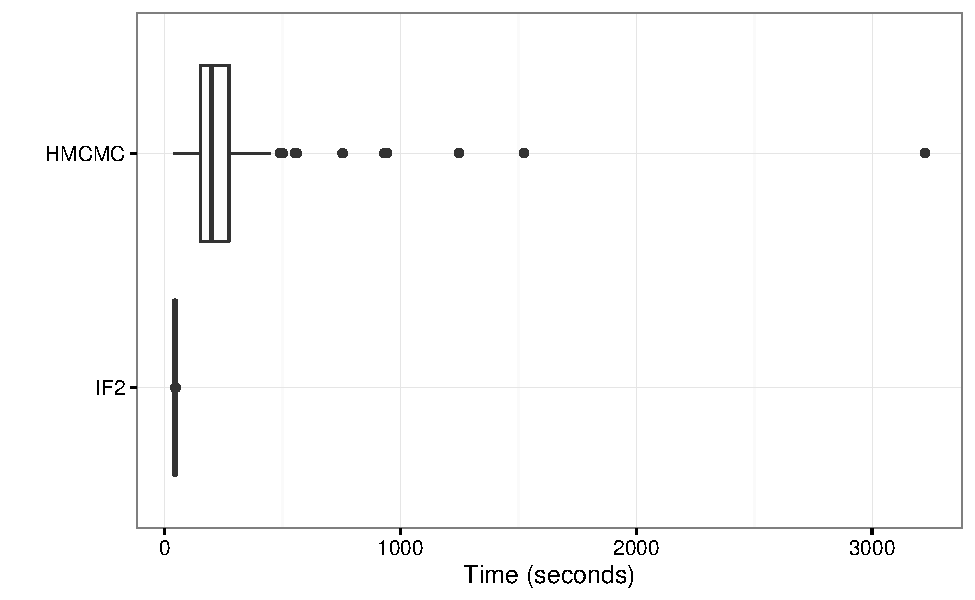
\includegraphics[width=0.8\textwidth]{./images/timeplot.pdf}
        \caption{Fitting times for IF2 and HMC, in seconds. The centre box in each plot shows the centre 50th percent, with the bold centre line showing the median. \label{sc1timeplot}}
    \end{figure}

    The average running times were approximately 45.5 seconds and 257.4 seconds for IF2 and HMC respectively, representing a 5.7x speedup for IF2 over HMC. While IF2 may be able to fit the model to data faster than HMC, we are obtaining less information; this will become important in the next section. Further, the results in Figure [\ref{sc1timeplot}] show that while the running time for IF2 is relatively fixed, the times for HMC are anything but, showing a wide spread of potential times.
